\chapter{Modelling the Whole Atrium}

In the previous chapter a modelling library suitable for simulation of single
cell and over 1D and 2D models of cardiac tissue was developed.
Single cell models are the base on which 1D and 2D models stand and 1D and 2D
models provide valuable insight into the behaviours of cardiac tissue in health
and disease.
It does not need to be said that the atrium is not 1D or 2D construct but is
instead a complex 3D structure.
This complexity can be seen internally, in that the atrium is comprised of several
separate tissue types with distinct electrophysiological behaviours and has
regions of differing conductivity.
It can also be seen in the gross physical structure, the atrium has a complex
topology with both holes for the venous and arterial openings, as well as
openings for the valves.
The simpler, often idealized, models constructed in the previous chapter
ignore (and in many cases, are incapable of showing) many of these complexities.
To provide insight into the atrium function on the whole organ level we must
therefore simulate the atrium as an organ.
A 3D model of the atrium requires a representation of the atrial geometry to
provide the topology of the atrium.
To model complexities with sufficient accuracy models of the
electrophysiologically distinct tissue types are also required as are
descriptions of the complex conductivities.


\section{Atrial Geometry}
\label{atrium:sec:geometry}

The atrial geometry used in the simulation studies presented here was based on
the visible human project female dataset.  The visible human dataset was
created from a pair of cadavers, set into wax and sliced into \mm{1}\ and
\mm{0.33}\ for the male and female bodies, respectively.  The geometric model
used here was extracted from the female dataset and so has a resolution of
\mm{0.33}.  The extracted geometry is segmented into different tissue types,
with distinct classifications for left and right atrium, the pectinate muscles,
the crista terminalis, the Bachmann bundle and the sino-atrial node, as shown in
figure \ref{atrium:geometry}.  The geometry has been used in numerous previous
simulation studies.  It was discretised via a finite differences approach, which
allows the whole atrium to be embedded in a block of $298\times269\times235$
nodes.  This gives it a total size of approximately 19 million total nodes,
although only approximately 1.6 million of those nodes correspond to excitable
cells.  The geometry also has simple fibre orientation in the pectinate muscles,
crista terminalis and Bachmann bundle.  The fibres are considered to always run
parallel to the local axis of the tissue bundle, as determined by principle
component analysis~\cite{Seemann2006}.

\section{Simulation Methods}
\label{atrium:sec:model}

\subsection{Atrial Model}

The electrical activity at each of the nodes was described by the equations of
the Courtemanche--Ramirez--Nattel (CRN) of the human atrial
myocyte~\cite{crn98}.  This model, as previously described, is a second
generation model. It has 21 state parameters, representing ionic gating activations
and inactivations and intracellular concentrations of ionic species.  In the
model, the total current, \ii{ion} is made up of the contributions of numerous
channels
\begin{equation}
\label{atrium:crn}
\ii{ion} = \ii{Na} + \ii{K1} + \ii{to} + \ii{Kur} + \ii{Ks} + \ii{Kr} +
\ii{Ca,L} + \ii{p,Ca} + \ii{NaK} + \ii{NaCa} + \ii{b,Na} + \ii{b,Ca}
\end{equation}
where \ii{Na}, \ii{K1}, \ii{to}, \ii{Kur}, \ii{Ks}, \ii{Kr}, \ii{Ca,L},
\ii{p,Ca}, \ii{b,Na} and \ii{b,Ca}\ represent ionic currents and \ii{NaK}\ and
\ii{NaCa}\ are ion exchangers.  As a second generation model, the CRN model also
has a detailed calcium handling system which can influence the action potential
via its influence on the intracellular calcium concentration.

In some atrial simulations it was desirable to incorporate details of
electrophysiological heterogeneity to represent the difference in electrical
behaviour between atrial myocytes and the other cellular types present in the
geometry, the pectinate muscles and crista terminalis.  The parameters used for
heterogeneity were based on measurements taken by Feng et al.~\cite{feng1998}
of the canine atrium.  These were converted to parameters for the CRN model by
Seemann et al.~\cite{Seemann2004} and have been used in several simulation
studies~\cite{Seemann2006,Stott2008}.  They are shown in
table~\ref{atrium:het_params}.

\subsection{Monodomain Equation}

To simulate the propagation of electrical activity over the finite difference
geometry previously described, the mono-domain equation is used to describe the
changes in $V$ in time, $t$, the trans-membrane voltage.
\begin{equation}
\label{atrium:monodomain}
\frac{\partial V}{\partial t} = \nabla\cdot D \nabla V - \frac{\ii{ion}}{C_{m}}
\end{equation}
where $D$ is a tensor representing the diffusivity of electrical potential, \ii{ion} is described by the
CRN model (\ref{atrium:crn}), $C_{m}$ is the membrane capacitance and all other
symbols have their usual meanings.  Equation (\ref{atrium:monodomain}) is
advanced in time via the forward euler method with a timestep of \ms{0.05}.  For
simulations with isotropic conductivity between nodes a 7-node approximation of
the differential operator is used.  When anisoptropy is present, a 27-node
approximation is used.

\subsection{Tissue Anisotropy}

The heart has a complex fibrous structure (Chapter 1), and this manifests
electrically as regions which have preferential conduction directions.
The preferential conduction directions show greatly increased conduction
velocities, sometimes by a factor of up to five~\cite{}.
The fibre structure and regions of preferential conduction are generally
considered much more important for the ventricles than for the atria.
The atria, or more specifically the right atrium, do possess several structures
with a definite direction of preferential conduction.
These are the crista terminalis, responsible for rapid conduction of the
depolarization wave to the atrio-ventricular node, the pectinate muscles and the
Bachmann bundle, the preferential pathway for conduction between the atria.
To determine the influence of anisotropic conduction on the propagation of the
electrical activity, we follow a method after Panfilov and
Keener~\cite{panfilov1995}.
In this method there is a unit vector, $\mathbf{f}$, defined at every point in
the tissue which has significant fibre orientation.
This unit vector defines a set of co-ordinate axes, in which the conductivity
tensor is diagonal
\begin{equation}
\label{atrium:dtilde}
\mathbf{\tilde{D}} =
\begin{pmatrix}
D_{\parallel} & 0 & 0\\
0 & D_{\perp} & 0\\
0 & 0 & D_{\perp}
\end{pmatrix}
\end{equation}
where $D_{\parallel}$ is the diffusion constant for conduction parallel to the
preferential direction of conduction and $D_{\perp}$ is the diffusion constant
for conduction perpendicular to this direction.
In this formulation it is assumed that there is no `sheet' structure which gives
a higher conduction velocity in one direction perpendicular to the main fibre
axis.
The diffusion tensor $\mathbf{\tilde{D}}$\ will only be diagonal in the
Cartesian co-ordinate system of the heart if the direction of preferential
conduction is parallel to one of the axes.
Therefore, to find the conductivity tensor in the global co-ordinate system,
$\mathbf{D}$, we need to find two transformation matrices $\mathbf{A}$\ and
$\mathbf{A^{T}}$\ such that
\begin{equation}
\label{atrium:d}
\mathbf{D} = \mathbf{A} \mathbf{\tilde{D}} \mathbf{A^{T}}
\end{equation}
To find $\mathbf{A}$\ it is possible to write out the involved rotations
explicitly, however an alternative method~\cite{fention2005}\ uses the fact that
$\mathbf{f}$\ and the two vectors orthogonal to it, $\mathbf{g}$\ and
$\mathbf{h}$\ are eigenvectors of $\mathbf{D}$.
These have the eigenvalues of $D_{\parallel}$\ and $D_{\perp}$.
The matrix $\mathbf{A}$\ is therefore an orthogonal matrix of the form
$\mathbf{A} = \left(\mathbf{f},\mathbf{g},\mathbf{h}\right)$ and so, using
(\ref{atrium:d}) $\mathbf{D}$\ can be written as
\begin{equation}
\label{atrium:dfgh}
\mathbf{D} = D_{\parallel}\mathbf{f}\mathbf{f^{T}} +
D_{\perp}\left(\mathbf{g}\mathbf{g^{T}} + \mathbf{h}\mathbf{h^{T}}\right)
\end{equation}
Using the fact that $\mathbf{A}\mathbf{A^T} = \mathbf{I}$ it is possible to
write
\begin{equation}
\label{atrium:dwithf}
\mathbf{D} = D_{\perp}\mathbf{I} + \left(D_{\parallel}-D_{\perp}\right)\mathbf{f}\mathbf{f^{T}}
\end{equation}
where $\mathbf{I}$\ is the identity matrix, and all other symbols are as defined
previously.
The directions of preferential conduction for the atrial geometry used in the
study were described by a pair of angles $\theta$\ and $\phi$\ representing the
orientation of the unit vector $\mathbf{f}$\ at each point in spherical polar
co-ordinates.
In cells with no assigned preferential conduction direction, the components of
$\mathbf{f}$\ were set to zero, giving a diffusion tensor of
\begin{equation}
\label{atrium:dnofibre}
\mathbf{D} =
\begin{pmatrix}
D_{\perp} & 0 & 0\\
0 & D_{\perp} & 0\\
0 & 0 & D_{\perp}
\end{pmatrix}
\end{equation}
which is the diffusion tensor for isotropic conduction.

\subsection{Computational Implementation}

The atrial geometry used in these studies is quite large, consisting of almost
19 million nodes.
As noted in \ref{atrium:sec:geometry}, only approximately 1.6 million of these
nodes correspond to active tissue--less than 10\% of the total.
The electrical activity at each node is represented by the CRN model and thus
requires 21 double precision numbers to be stored, representing the state
variables of the model.
The memory requirements of the model may be significantly reduced by storing
state variables, and where anisotropy is present the diffusion tensor, only for
the active nodes.
This reduces the memory requirements for storing the state variables from
approximately \unit{2.9}{GB}\ to \unit{256}{MB}.
A further simplification may be obtained by decomposing the geometry into a
linear array, containing the 7 or 27 neighbours of the active nodes to be used
in the diffusion tensor approximation.
The geometry and state information can therefore be represented by one linear
array of cellular states, one linear array used as a `map' and optionally, one
linear array representing the components of $\mathbf{D}$.
This linear data structure is very easy to parallelize on a shared memory
system.

The parallelization was accomplished through the use of the OpenMP shared
memory parallelism library~\cite{OpenMP}.
The system was then solved on 1 node of the Horace supercomputer on a total of 8
cores.
The linear array of active nodes was divided equally between the 8 cores, with
each core solving (\ref{atrium:crn}) for all nodes its assigned section of the
array.
A snapshot of the trans-membrane potentials at each of the active node sites was
output every \ms{2.5}\ of simulated time.
Simulation of \unit{1}{s}\ of atrial activity took XXXX hours.
A parallel fraction of XXXX was attained, indicating that almost all of the
workload was effectively distributed over the 8 cores.

\section{Mutation in KCNQ1: A Simulation Study}

Atrial Fibrillation (AF) is the most common arrhythmia in the developed world.
It is a self-promoting condition, with paroxysmal AF episodes frequently
degenerating into chronic and even permanent AF.
Clinically, AF patients show an erratic and high frequency ECG.
At the cellular level, AF is characterised by an abbreviated action potential
(AP) which has no plateau phase and poor heart rate adaptability.
The mechanisms through which AF influences the heart are complex, but the
remodelling of the cellular electrophysiology is believed to contribute to
reduced ERPs and through that, favour the formation of stable, long lived
spiral waves and organ level microwavelet re-entry.
AF is often preceeded by congestive heart failure, cardiomegaly and other
structural cardiac diseases, but there are significant numbers of suffers with
no such structural defects.
There is also evidence of a genetic predisposition to AF, which is sometimes
termed Familial Atrial Fibrillation.
Several gene mutations have been causally implicated for AF, leading to AF
which manifests both with and without associated structural cardiac disorders.
The ion channels associated with the repolarisation reserve (\ii{K1}, \ii{Kr},
\ii{Ks}) are particularly important to the genesis of AF.
Alterations in functions, gating and kinetics have been implicated in both short
and long QT syndromes.
The \ii{Ks}\ channel has very slow activation kinetics which enable it to
regulate cardiac APs over a wide range of plateau voltages.
Mutations in the \ii{Ks}\ channel are common.
Several mutations in the $\alpha$-subunit, coded for by the KCNQ1 gene, of the
\ii{Ks}\ channel have been identified including both loss-of-function and
gain-of-function, leading to the SQT syndrome and to AF.
Chen et al. studied a four generation Chinese family with hereditary persistent
AF.
They identified a missense mutation at nucleotide 418 from adenine to guanine
resulting in a change from serine to glycine at position 140 (S140G mutation of
\ii{Ks}).
This missense mutation lead to a large gain-of-function which included changes
in the channel kinetics.
It has been hypothesised that these changes in the function of the \ii{Ks}\
channel in the human atrium result in abbreviations of both APD and ERP and thus
provide an appropriate substrate for the genesis of AF.

This study had two goals: To construct a computer model of the available
experimental data from Chen et al. and to then use this model to quantify the
effects of the mutation through the use of cellular, 1D, 2D and 3D models

\subsubsection{Modelling the Mutation}

This study, as in the previous chapter, uses the CRN model, developed by
Courtemanche et al.~\cite{CRN1998}\ for simulation of the human atrial action
potential.
As a biophysically detailed model with 21 state variables and numerous ion
channels it is ideal for use in mutation studies.
The CRN model has individual descriptions of several $K^{+}$\ currents.
These include the time-independent potassium current, \ii{K1}, the ultra-rapid
potassium current, \ii{Kur}, the transient outward current, \ii{to}\ and the
rapid and slow delayed rectifier currents, \ii{Kr}\ and \ii{Ks}.
The latter current is modulated by the mutation and is described in the control
CRN cell by
\begin{equation}
\label{atrium:iks_con}
\ii{Ks} = g_{Ks}x_{s}^{2}\left(V-E_{K}\right)
\end{equation}
where $g_{\tiny{Ks}}$\ is the channel conductance (\unit{0.129}{nS/pF}), $x_{s}$\ is
the activation variable and $E_{K}$\ is the $K^{+}$\ reversal potential, found
through the Nernst potential.

\subsubsection{Simulation of the S140G mutation of KCNQ1 I-V relationship}

The Chen et al.~\cite{Chen2003} study determined that the most likely cause of
familial AF was was the S140G mutation of the KCQN1 gene, which forms part of
the $\alpha$-subunit of the \ii{Ks}\ channel.
The gene was transfected into COS7 cells along with the second component of
the $\alpha$-subunit, KCNE1, in both normal (WT) and mutated type (MT).
The transfected cells were used to perform voltage clamp experiments.
The clamp protocol used is shown in Figure~\ref{atrium:iks:vc},A.
This is the experimental protocol used by Chen et al.~\cite{Chen2003}.
The cell was held at a holding potential of \mv{80} for \unit{0.5}{s}\ before
being held at \mv{10}\ steps between \mv{-130}\ to \mv{50}\ for \unit{3}{s}.
The voltage steps were followed by a \mv{-40}\ holding potential, applied for
\unit{1}{s}.
The values of \ii{Ks} at the end of the step voltages were plotted against the
step voltages to determine  I-V relationships for WT
and MT cells, shown in Figure~\ref{atrium:iks:vc},B (points with errors) and
current traces, shown in Figure~\ref{atrium:iks:vc},C and D for WT and MT,
respectively.

\begin{figure}
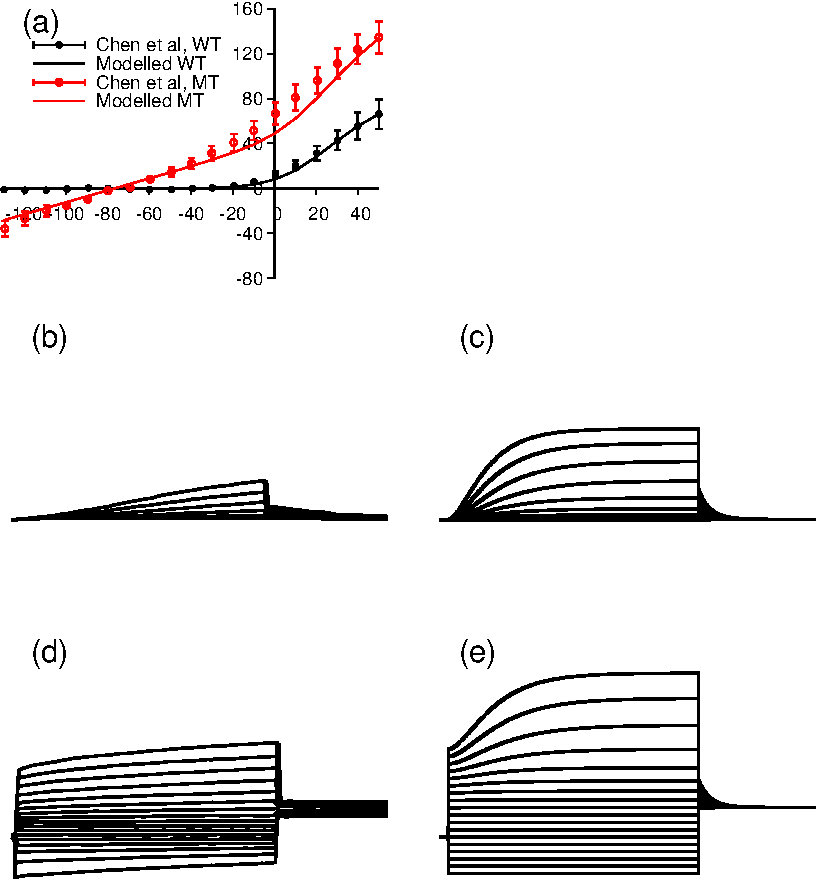
\includegraphics{figures/atrium/iks/figures/01_IV}
\caption[KCNQ1 mutation in IKs, experimental data]{
\label{atrium:iks:vc}
\textbf{A} Voltage clamp protocol used by Chen et al.~\cite{Chen2003}.
\textbf{B} Experimental WT (black, closed circles) and MT (red, open circles)
I-V relationships recorded by Chen et al.  Simulated I-V curves for WT (black
lines) and MT (red lines).  Modelled curves are scaled to experimental points
based on the WT current density at \mv{50}.
\textbf{C} Experimental current traces for WT.
\textbf{D} Simulated current traces for WT.
\textbf{E} Experimental current traces for MT.  Note the instantaneous
activation, and the significant inward current at negative clamp potentials.
\textbf{F} Simulated current traces for MT.
}
\end{figure}

The I-V relationship shows that the mutation causes a gain-of-function across
all the clamp potentials.
It also reveals that the mutation appears to cause an inward current at negative
potentials.
The current traces suggest a drastic change in the kinetics of the \ii{Ks}\
channel with a significant component of the current being activated immediately.
The addition of a leakage component to (\ref{atrium:iks_con}) allowed simulation
of \ii{Ks}\ characteristics which closely matched the experimental data.
Under MT conditions, the new total current \iip{Ks}\ was described by
\begin{equation}
\label{atrium:iks_mut}
\iip{Ks} = \ii{Ks} + \varphi g_{Ks}x\left(V-E_{rev}\right)
\end{equation}
where \ii{Ks}\ is (\ref{atrium:iks_con}), $\varphi$\ is a multiplicative parameter
from with values between 0 and 1, $g_{Ks}$ is as in (\ref{atrium:iks_con}) and
$E_{rev}$\ is the reversal potential of the leakage component.
The reversal potential was estimated from the experimental I-V relationships to be
\mv{-76.3}.
The inclusion of the $\varphi$\ parameter allowed the simulation of several
intermediate mutant states, representative of a heterozygous mutation.
Setting $\varphi = 1$\ and following the voltage clamp protocol shown in panel A
of Figure~\ref{atrium:iks:vc}\ the I-V relationship of \ii{Ks}\ was simulated to
provide a good match to experimental data shown as the lines in panel B of
Figure~\ref{atrium:iks:vc}.
Also shown are the simulated current traces elicited by the voltage clamp
protocol in panels D and F.
The non-gated leakage component of \iip{Ks}\ sufficiently accounts for the
changed current density and kinetics.

\subsubsection{Simulation Protocols}

To assess the effects of the mutation on human atrial myocytes, cellular models
including the modified \iip{Ks}\ described by (\ref{atrium:iks_mut}) were used
in a number of simulation protocols, as described in Chapter 2.
Initially the \apd\ was evaluated under conditions corresponding to $\varphi =
0$\ (WT) and $\varphi = 1$\ (MT).
Under such conditions, the induced \apd\ shortening was found to result in
un-physiological \apd\ values, shown in Figure \ref{atrium:iks:apd}.
Therefore a pair of heterozygous cases, corresponding to $\varphi = 0.10$\
(HT10) and $\varphi = 0.25$\ (HT25) were created and used in the evaluation of
the mutation's effects.

Using the models and protocols described in Chapter 2 the \apdr, ERP\emph{r}, VW,
CV\emph{r}, SVW and the dynamic behaviours of spiral waves were evaluated for
the WT, HT10 and HT25 cases.
For the 3D simulations, the model described in Sections
\ref{atrium:sec:geometry}\ and \ref{atrium:sec:model}\ was used.
Since the intention was just to investigate the influence of the mutation, the
model was used without tissue anisotropy.
The mutation was applied homogeneously with the electrical activity at all
nodes described by either the WT or HT10 cells.
An atrial model of nodes described by HT25 cells did support stable conduction
and so it was not used in the 3D studies.
There was no heterogeneity introduced to account for the differing cell types
present in the human atrium.
To examine the behaviour of scroll waves under WT and HT10 conditions a protocol
analogous to the wave-break protocol described for 2D sheets of tissue was
used~\cite{Kharche2007}.
The protocol is illustrated in Figure~\ref{atrium:iks:scroll_init}.
\begin{figure}
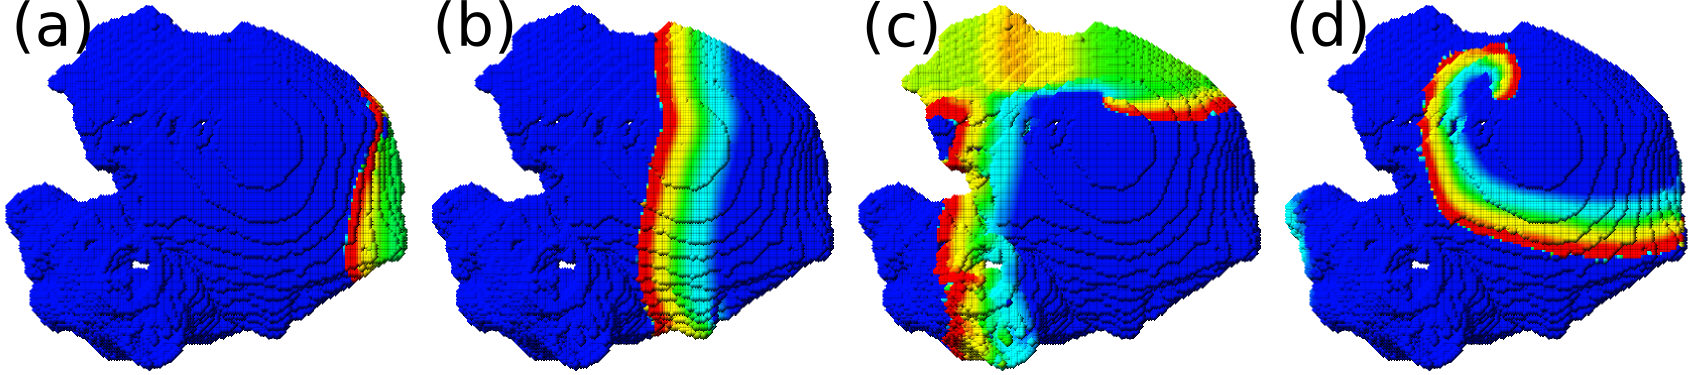
\includegraphics{figures/atrium/iks/scrollhowto}
\caption[Initiating a Scroll Wave]{
\label{atrium:iks:scroll_init}
Stimulus protocol used to initiate a scroll wave.
\textbf{A} One extreme of the atrial model is stimulated
\textbf{B} The excitation is allowed to propagate
\textbf{C} An S2 stimulus is delivered by clamping a section of the tissue, here
the lower quarter.
\textbf{D} A scroll wave begins on the wall of the right atrium.
}
\end{figure}
First, a small number of cells are simulated at one extreme of the atrial model.
The excitation is allowed to propagate through the model until the S2 stimulus
is delivered.
The S2 stimulus is delivered via briefly clamping a section of the atrial model to
\mv{50}\ and then releasing the clamp.
A correctly timed S2 stimulus results in a scroll wave on the wall of the right
atrium.
After initiation, the models were simulated until activity ceased or until
\unit{6}{s}\ of simulated time had elapsed.

\subsubsection{Changes in \apd\ due to S140G mutation}

The effect of an increase in the leakage current parameter were investigated.
This was done using the standard \apd\ protocol and varying $\varphi$\ between
0 and 1.
Variation in \apd\ as $\varphi$\ is altered is shown in
Figure~\ref{atrium:iks:aps},A.
Representative APs are shown in Figure~\ref{atrium:iks:aps},B.
The \apd\ under Control conditions (WT) was seen to be \ms{312.0}.
Progressive mutation decreased the \apd\ to \ms{150.5}\ in HT10 case and
\ms{79.3}\ in HT25 case.
Under homozygous conditions, $\varphi = 1$\, the \apd\ was seen to be \ms{22.4}.
Figure~\ref{atrium:iks:aps},B shows the inclusion of the mutant channel causes
the changes in morphology associated with none of the mutant types having a
plateau region.
Inclusion of the mutant channel decreased the upstroke velocity of the AP from
\unit{217.1}{V/s}\ in WT, to \unit{214.0}{V/s}\ in HT10 and \unit{208.6}{V/s}\
in HT25.
The upstroke velocity in the homozygous case was \unit{192.0}{V/s}.

\subsubsection{\apdr\, ERP\emph{r}, CV\emph{r} and VW}

Figure~\ref{atrium:iks:apdretal},A shows the current profiles of \ii{Ks} over the course of
an AP which correspond to the AP traces shown in Figure~\ref{atrium:iks:aps},B.
\ii{Ks}\ is seen to increase considerably in both the HT10 and HT25 cases
compared with the WT case.
The leak also changes the morphology of the current profile to one showing
almost instant activation in HT10 and HT25 cases, compared to the slow
activation in WT.
The \apdr\, Figure~\ref{atrium:iks:apdretal},B, reflects the decreased \apd\ with
the restitution curves considerably flattened for both the mutant cases.
The maximal slopes of the \apdr\ were measured to be 1.9, 0.78 and 0.56 in cases
WT, HT10 and HT25 respectively.
The ERP\emph{r}\ curves, Figure~\ref{atrium:iks:apdretal},C, also reflect the
reduced \apd\.
At an S1 interval of \ms{1000}\ the ERP was found to be \ms{XXXX}\ in WT,
\ms{XXXX} in HT10 and \ms{XXXX} in HT25.
In addition, the mutant cases supported excitation at much lower S1 intervals
(or higher pacing rate) compared to the control case.
The minimum S1 interval sustained during the ERP\emph{r}\ calculations was
\ms{XXXX}\ in WT, \ms{XXXX} in HT10 and \ms{XXXX} in HT25.
The solitary wave CV was not altered considerably by the mutation (\cms{26.7}\
in WT c.f. \cms{27.0} in HT25).
The CV\emph{r}\, Figure~\ref{atrium:iks:apdretal},D, curves confirm the findings
of the ERP\emph{r}\ calculations, that the mutant case supports successful
excitation after a considerably reduced S2 interval.
The minimum S2 interval which still allowed the test stimulus to propagate was
found to be \ms{318.9}\ in WT, \ms{181.2}\ in HT10 and \ms{120.4}\ in HT25.
Vulnerability to premature excitation was relatively unaffected by the mutation,
having a value of approximately \ms{XXXX} in all cases.
